

\subsection{ROC - AUC (Receiver Operating Characteristic curve and Area Under the Curve)}

\begin{figure}[H]
    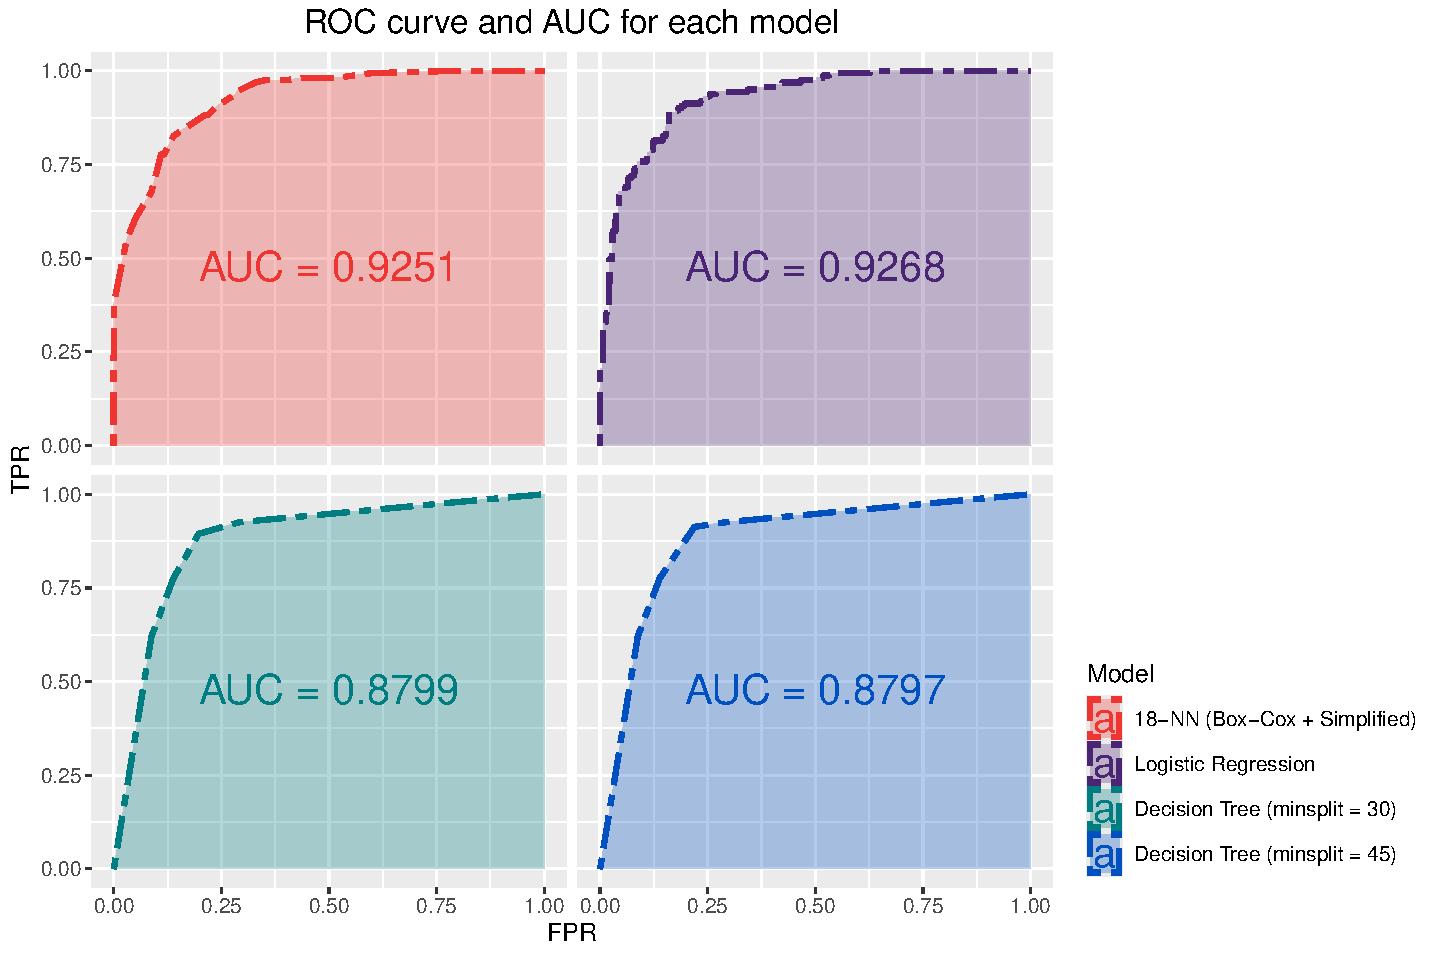
\includegraphics[width=\linewidth]{40.ROCs.pdf}
    \caption{\centering ROC curves and AUC for each model}
\end{figure}

Surprisingly, \( 19 \)-NN and logistic model produce similar ROC curves, despite having different modelling methodologies. It is less so for decision trees, as their alike curves can be explained by the analogous inner mechanisms of their structure.

In terms of AUC score, \( 19 \)-NN and logistic model give impressive scores of \( 0.9245 \) and \( 0.9268 \) respectively, whilst decision trees only yield less impressive scores from \( 0.8797 \) to \( 0.8799 \). The former models excel by considering exhaustive combinations of features, whilst the latter models suffer from overgeneralisation by only considering the most important features and skipping the details.


